\documentclass[11pt]{article}

\usepackage[margin=1in]{geometry}
\usepackage{amsmath,amssymb}
\usepackage{graphicx}
\usepackage{booktabs}
\usepackage[numbers,sort&compress]{natbib}
\usepackage{microtype}
\usepackage{xcolor}
\usepackage[colorlinks=true,linkcolor=blue!60!black,citecolor=blue!60!black,urlcolor=blue!60!black]{hyperref}

\hypersetup{
  pdftitle={SwitchSync Markets: A Preregistered Synthetic Stress Test of Switching Synchronization as a Financial-Network Mechanism},
  pdfauthor={AUTHOR METADATA PENDING (placeholder; human author not yet provided)},
  pdfsubject={Preregistered, fully synthetic stress test of switching-induced synchronization as a financial-network mechanism; confirmatory outcomes inconclusive or failed; no real market data},
  pdfkeywords={synchronization, temporal networks, link switching, master stability function, preregistration, financial networks, identifiability, FitzHugh--Nagumo}
}

\graphicspath{{figures/}}

\newcommand{\Tswt}{T_{\mathrm{swt}}}
\newcommand{\NIL}{N_{\mathrm{IL}}}

\title{SwitchSync Markets: A Preregistered Synthetic Stress Test of Switching
Synchronization as a Financial-Network Mechanism}

\author{[AUTHOR NAME PENDING --- PLACEHOLDER]\thanks{PLACEHOLDER: the human
author's name, affiliation, contact email and (optional) ORCID have not yet
been provided and are deliberately \emph{not} fabricated; this release
candidate is blocked on that metadata and on the license choice
(\texttt{PAPER\_RC\_BLOCKED\_ON\_AUTHOR\_METADATA\_AND\_LICENSE}). Repository:
\texttt{switchsync-markets}. This is a fully synthetic, preregistered study;
no real market data were used at any stage.}}

\date{July 2026}

\begin{document}
\maketitle

\begin{abstract}
Dynamic link switching can induce stable synchronized states in sparse
multilayer networks of chaotic oscillators \citep{eser2025switching}. We ask
whether this mechanism admits a mathematically faithful and observationally
identifiable translation to financial temporal networks, where cross-venue
arbitrage channels open and close over time. Rather than fitting market data,
we preregistered falsifiable gates and executed them \emph{exactly once} on
frozen synthetic systems: a two-layer FitzHugh--Nagumo (FHN) benchmark and a
linear stochastic surrogate with paired switching schedules, under a frozen
statistical decision contract (exact sign test plus a preregistered effect
band). The calibrated demonstration gate passed: at $\sigma_{12}=1.5$, $N=40$,
fast switching synchronizes the layers and slow switching does not. Every
translation-relevant gate, however, failed to establish its claim. The
switching-versus-static advantage was directionally consistent (8/8 positive
paired differences, $p=0.0078$) but below the preregistered magnitude band
(INCONCLUSIVE/TIE); the strict comparison against the average graph and the
best frozen static comparator is not interpretable under the frozen hierarchy,
with diagnostically negative differences in all eight seeds. Because G1-weak
did not pass, G2 was formally NOT\_INTERPRETABLE; its diagnostic order
statistic was non-significant. Robustness stages never exceeded their bands,
and observational identifiability failed outright (precision and recall
$\approx0.35$ against a 0.6 bar), with asynchronous, last-observation-carried-forward
sampling collapsing the contraction correlation from $0.948$ to $0.010$
(an Epps-like degradation \citep{epps1979comovements}). We conclude that the
financial translation is not supported for empirical or operational
development under the preregistered criteria. This negative result does not
refute the mathematics of the seed paper; it constrains what that mechanism
can be expected to deliver as a measurable, decision-relevant object in
financial data. No real market data were used.
\end{abstract}

\section{Introduction}
\label{sec:intro}

In a recent arXiv preprint, Eser, Medeiros, Riza and Engel showed that
switching a sparse set of inter-layer links --- rather than keeping them fixed
--- can stabilize inter-layer synchronization in two-layer networks of chaotic
FitzHugh--Nagumo oscillators, with faster switching more effective
\citep{eser2025switching,eser2021edges}. The mechanism is attractive to a
financial modeler: markets trade the \emph{same} economic asset on multiple
venues; the cross-venue ``links'' (arbitrage channels, shared market makers,
funding connections) are sparse, come and go over time, and venue prices are
observed to lock together or drift apart episodically
\citep{hasbrouck1995one,alexander2020bitmex,baur2019price}. If switching-induced
synchronization survived translation, ``which channels are open, in what order,
and at what rate'' would be a structural, measurable determinant of cross-venue
price locking, distinct from aggregate connectedness measures
\citep{diebold2009measuring,diebold2014network,billio2012econometric}.

That conditional is precisely what this paper tests, and the honest answer is
negative under our preregistered criteria. Three failure modes make naive
translations of synchronization results to finance unreliable: (i) fast-switching
averaging theory implies that rapidly switched networks behave like their
time-averaged counterpart
\citep{belykh2004blinking,stilwell2006sufficient,hasler2013dynamics}, so an
apparent ``switching effect'' may carry no information beyond the average
graph; (ii) small ensembles invite effect-size inflation, so magnitude criteria
must be fixed before observing data; and (iii) even a real mechanism is useless
to empirical finance if it cannot be identified from asynchronously observed
prices \citep{epps1979comovements,scholes1977estimating,hayashi2005covariance}.
We therefore preregistered a gate hierarchy with frozen grids, seeds,
estimands and decision rules; froze the code and configuration under
content-addressed manifests; executed the suite exactly once under an
auditable custody protocol; and committed the sealed outputs byte-for-byte.

Section~\ref{sec:results} reports the outcomes
(Table~\ref{tab:gates}, Figure~\ref{fig:summary}): the mechanism demonstrably
operates in a calibrated synthetic setting (G0B PASS), but no
translation-relevant gate established its claim, and identifiability failed.
Throughout, we separate \emph{confirmatory} preregistered outcomes,
\emph{diagnostic} quantities that the frozen hierarchy declares
non-interpretable, \emph{descriptive} observations, and \emph{conjecture}.

\section{Mathematical Background}
\label{sec:background}

\paragraph{Synchronization and master stability.}
For diffusively coupled identical oscillators, the stability of the
synchronous state is governed by the transverse (conditional) Lyapunov
exponents of the variational dynamics
\citep{pecora1990synchronization,pecora1998master}. On a static graph the
problem factorizes into a master stability function (MSF) evaluated at the
Laplacian eigenvalues.

\paragraph{Time-varying coupling.}
When the coupling network varies in time, the static MSF picture survives
exactly only in special cases, e.g.\ commuting coupling matrices
\citep{boccaletti2006commutative}. In the fast-switching regime, averaging
results guarantee synchronization whenever the \emph{time-averaged} network
synchronizes \citep{belykh2004blinking,stilwell2006sufficient}, with
finite-rate deviations bounded by blinking-system theory
\citep{hasler2013dynamics}. Consensus theory gives the discrete-time
counterpart: joint connectivity over time windows suffices
\citep{jadbabaie2003coordination,olfatisaber2004consensus,moreau2005stability,renbeard2005consensus}.
Empirically, rapidly switched links promote synchronization in a range of
models \citep{kohar2014synchronization,zhou2019random}; see
\citep{ghosh2022synchronized} for a survey, \citep{holme2012temporal} for the
temporal-network formalism, and \citep{jardon2024persistent} for rigorous
conditions under time-dependent diffusive coupling.
\emph{Crucially}, temporal networks \emph{can} outperform any static network of
equal resource budget in designed settings \citep{zhang2021designing}, so
``switching never beats the average'' is not a theorem; whether it holds in a
given ensemble is an empirical question --- the one our G1/G2 gates formalize.

\paragraph{The seed mechanism.}
The seed paper \citep{eser2025switching} couples two ring layers of chaotic
FHN oscillators through a sparse, randomly re-drawn set of inter-layer links
with dwell time $\Tswt$, and reports that sufficiently fast switching induces
stable inter-layer synchronization at link densities where static sparse
coupling fails; its predecessor \citep{eser2021edges} maps the edges of
inter-layer synchronization under time-switched links.

\section{Financial-Network Translation and Its Assumptions}
\label{sec:translation}

The proposed reading maps: layers $\to$ venues quoting the same asset;
inter-layer synchronization $\to$ cross-venue price locking (conceptually a
cointegration-like common component \citep{gonzalo1995estimation}); the sparse
switching link set $\to$ the currently active arbitrage/market-making
channels; the switching rate $\to$ channel-rotation speed. Under this reading,
price-discovery leadership that migrates between venues over time
\citep{hasbrouck1995one,baur2019price,alexander2020bitmex} is the observable
trace of channel switching.

This translation embeds strong assumptions, each of which can independently
fail without contradicting the seed mathematics:
\begin{enumerate}
  \item \textbf{Mechanism transfer:} the contraction advantage of switching
  must survive in dynamics that are not two-layer chaotic FHN rings --- here
  probed with a linear stochastic surrogate (Section~\ref{sec:design}).
  \item \textbf{Beyond-average content:} the switching structure must matter
  \emph{beyond} the time-averaged connectivity; otherwise standard aggregate
  connectedness measures \citep{diebold2009measuring,diebold2014network,engle2002dynamic}
  already capture everything, and correlation-based ``regime'' readings risk
  the classic confound between interdependence and heteroskedasticity
  \citep{forbes2002no}.
  \item \textbf{Identifiability:} the active channel set must be recoverable
  from observed prices, after removing common factors
  \citep{fan2013large,barigozzi2017network} and despite asynchronous
  observation \citep{epps1979comovements,hayashi2005covariance,scholes1977estimating}.
\end{enumerate}
We emphasize what the translation, even if successful, would \emph{not} give:
a trading signal, a backtest, or any claim about market causality. None is
made anywhere in this paper.

\section{Hypotheses and Preregistered Gates}
\label{sec:gates}

The preregistration (v8; hashes in Appendix~\ref{app:audit}) freezes a gate
hierarchy. Each gate has a frozen estimand, grid, seed block and decision
rule; outcomes are PASS / FAIL / INCONCLUSIVE / EXECUTION\_INVALID, with
NOT\_INTERPRETABLE for sub-gates whose interpretability is conditional.

\begin{description}
  \item[G0A (exact reproduction; expensive).] Reproduce the paper-scale regime
  ($\sigma_{12}=0.1$, $N\in\{100,200,400\}$). \emph{Not run} in this study
  (Section~\ref{sec:results}).
  \item[G0B (calibrated demonstration).] At a re-calibrated coupling
  ($\sigma_{12}=1.5$, $N=40$), fast switching ($\Tswt\le 10$) must synchronize
  and slow switching ($\Tswt\ge 160$) must not. \emph{This is a qualitative
  demonstration of the mechanism, never an exact reproduction.}
  \item[G0C (minimal MSF).] In a minimal two-node transverse-stability
  computation with switched anti-phase coupling channels, the stability onset
  must depend on $\Tswt$.
  \item[G1-weak.] In the surrogate, the selected switching arm must beat the
  equal-instantaneous-density static-sparse comparator on paired evaluation
  seeds.
  \item[G1-strict.] The arm must beat \emph{both} the average-graph operator
  and the best static subset from a frozen candidate set
  (``best-of-frozen-candidate-set''; the admissible universe
  $\binom{24}{6}=134{,}596$ is \emph{not} searched, so no claim about the best
  admissible static is possible). Interpretable only if G1-weak passes.
  \item[G2 (temporal order).] The ordered schedule must differ from the median
  over frozen order permutations of the same epoch multiset
  (permutation-median comparator + cross-seed sign test). Interpretable only
  if G1-weak passes.
  \item[G3 (robustness).] The weak advantage must persist under implemented
  stresses (heterogeneity, directedness, signed weights); PASS requires the
  faithful and mild-heterogeneity stages to pass.
  \item[G4 (identifiability).] A past-only estimator must recover the active
  channel set from noisy observations of the surrogate (precision and recall
  $>0.6$), track contraction (correlation $>0.5$, same-realization ground
  truth), and beat a factor-confounded baseline; tested under synchronous and
  asynchronous (LOCF) observation.
\end{description}

\section{Synthetic Models and Experimental Design}
\label{sec:design}

\paragraph{FHN benchmark (G0A/G0B).}
Two ring layers of $N$ FitzHugh--Nagumo oscillators
($\epsilon=0.05$, $a_{\mathrm{odd}}=0.87$, $a_{\mathrm{even}}=0.97$, rotational
coupling angle $\phi=\pi/2-0.1$, intra-layer coupling $\sigma_{\mathrm{intra}}=0.1$,
nearest-neighbor ring) are coupled through a diffusive inter-layer term of
strength $\sigma_{12}$ on a switching subset of $\NIL=N/4$ mirror pairs,
re-drawn uniformly at random every $\Tswt$ time units (RK4, $\mathrm{d}t=0.01$).
Synchronization is declared by a \emph{deterministic} per-seed criterion: the
tail time-average (final 25\%) of the inter-layer error $E_{12}$ must fall
below the frozen threshold $0.02$ (this threshold is not an effect-band floor;
see Section~\ref{sec:contract}). G0B uses $N=40$, $\sigma_{12}=1.5$, total time $800$,
$\Tswt\in\{2,\dots,300\}$, five seeds per cell.

\paragraph{Minimal MSF system (G0C).}
A minimal $N=2$ transverse-stability computation integrates the variational
dynamics along the synchronized trajectory under smoothly switched anti-phase
coupling channels ($\lambda_\perp=2$, smoothing $\alpha=5$), scanning
$\sigma\in\{0.05,0.15,0.3,0.5,0.8\}$ and $\Tswt\in\{11,25,100,135\}$. The
anti-phase channel prerequisite is verified before any science value is
computed.

\paragraph{Linear stochastic surrogate (G1--G4).}
To probe mechanism transfer outside chaotic FHN dynamics we use a linear
stochastic surrogate: two coupled layers of $N=24$ nodes whose inter-layer
difference evolves through a sequence of linear difference-step maps
(local spectral radius $1.04$, i.e.\ intentionally near-unstable between
couplings; coupling gain $\kappa=0.6$ on open channels; weak intra-layer
mixing $0.06$). The estimand is the contraction rate $\gamma$ of the ordered
product of the step maps over a frozen horizon $H=240$: $\gamma>0$ means the
venue-difference (basis) process contracts. Schedules are \emph{paired}: all
comparators share the same base snapshots (six snapshots of six channel pairs)
per seed, so differences isolate scheduling. The rate arms (fast /
intermediate / slow) cycle the snapshot sequence $20/5/1$ times within $H$.
The switching arm and the best static candidate are selected on eight
selection seeds and frozen \emph{before} the eight disjoint evaluation seeds
are opened; the static candidate set is the union of the base snapshots and a
frozen 200-draw random search (248 candidates here).

\paragraph{Identifiability testbed (G4).}
On the same surrogate (horizon 600, fast dwell 6), a past-only,
factor-free estimator based on venue differencing (window 8, observation noise
$0.05$) reconstructs the active channel set; it is compared against a
deliberately factor-confounded level-correlation baseline
(cf.\ \citep{fan2013large,barigozzi2017network} for factor-removal rationale).
Ground truth is the same realization's schedule. Observation is either
synchronous (1:1) or asynchronous with last-observation-carried-forward at
ratio 1:3 --- an \emph{asynchrony/LOCF (Epps-like degradation)} design, not a
causal demonstration of the Epps effect.

\paragraph{Custody.}
All grids, seeds, tolerances and decision rules above were frozen in
preregistration v8 and its bound execution contract v6 before execution; the
code and configuration were sealed by a content-addressed freeze manifest
(v8), and the suite ran exactly once under an authorization token whose
SHA-256 is recorded in every artifact (Appendix~\ref{app:audit}).

\section{Statistical Decision Contract}
\label{sec:contract}

Every paired comparison uses one shared, frozen rule. For paired differences
$d_1,\dots,d_n$ ($n=8$ evaluation seeds; differences with $|d|\le 10^{-12}$
dropped and disclosed):
\begin{enumerate}
  \item an exact two-sided sign test on the non-zero $d_s$ at $\alpha=0.05$
  (with $8/8$ equal signs, $p = 2\cdot\binom{8}{0}/2^8 = 0.0078$, so $n=8$
  \emph{can} reach significance);
  \item a preregistered \emph{effect band}
  $b=\max\!\big(3\,\hat{\sigma}_{\mathrm{ddof}=1},\ \text{floor}\big)$, with
  frozen floors: $0.02$ for paired differences of the surrogate contraction
  rate $\gamma$, and $0.05$ for the identifiability margin over the baseline
  (G4);
  \item decision: if $p\ge\alpha$ $\to$ INCONCLUSIVE (NOT\_SIGNIFICANT); else
  if $\bar d> b$ $\to$ PASS; else if $\bar d<-b$ $\to$ FAIL; else
  $\to$ INCONCLUSIVE (TIE).
\end{enumerate}
The G0B synchronization criterion (tail-averaged $E_{12}<0.02$) is a
\emph{deterministic threshold} applied per seed, not an effect-band floor, and
plays no role in the paired rule; the two $0.02$ values are numerically equal
but contractually distinct objects. A bootstrap interval (2{,}000 resamples,
frozen seed) is reported as a \emph{descriptor only} and plays no role in
decisions. A global failed-seed
policy invalidates any cell with more than 20\% technical failures; the
executed run had \textbf{zero} failures, non-finite values or dropped seeds.
The hierarchy is frozen: G1-strict and G2 are interpretable only if G1-weak
passes; otherwise their computed values are reported as diagnostics and are
not gate outcomes.

\section{Results}
\label{sec:results}

Table~\ref{tab:gates} and Figure~\ref{fig:summary} summarize the outcomes of
the single authorized run (sealed attempt \texttt{1baa47da06fede2a});
Table~\ref{tab:inference} lists every decision statistic.

% Required preregistered results table. Source: frozen JSON reports of sealed
% attempt 1baa47da06fede2a (freeze v8). Byte hashes in Appendix A.
\begin{table}[t]
\centering
\caption{Preregistered gate outcomes of the single authorized cheap-suite run
(attempt \texttt{1baa47da06fede2a}, execution freeze v8). ``Confirmatory'' outcomes
follow the frozen decision contract of Section~\ref{sec:contract}; quantities marked
``diagnostic'' are reported but are, by the preregistered hierarchy, not gate
outcomes. Zero technical failures, non-finite values or dropped seeds occurred in any
gate.}
\label{tab:gates}
\resizebox{\linewidth}{!}{%
\begin{tabular}{@{}llll@{}}
\toprule
Gate & Question (frozen) & Verdict & Status \\
\midrule
G0A & exact paper-scale reproduction & NOT\_RUN & outside cheap-suite scope \\
G0B & calibrated small-$N$ demonstration & \textbf{PASS} & confirmatory (demonstration only) \\
G0C & minimal MSF $T_{\mathrm{swt}}$-dependence & INCONCLUSIVE & confirmatory \\
G1-weak & switching beats equal-density static & INCONCLUSIVE (TIE) & confirmatory \\
G1-strict & beats average graph and best frozen static & NOT\_INTERPRETABLE & diagnostic only \\
G2 & temporal order beyond the multiset & NOT\_INTERPRETABLE & diagnostic only \\
G3 & robustness of the weak advantage & INCONCLUSIVE & confirmatory \\
G4 & observational identifiability & \textbf{FAIL} & confirmatory \\
\bottomrule
\end{tabular}}
\end{table}


\begin{figure}[t]
  \centering
  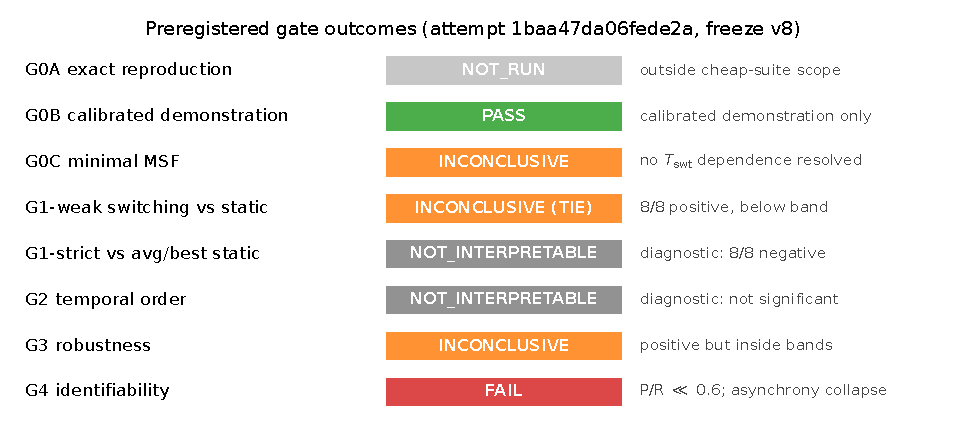
\includegraphics[width=0.88\linewidth]{fig_gate_summary.pdf}
  \caption{Gate summary. Grey chips mark quantities that the frozen hierarchy
  declares non-interpretable (diagnostic only).}
  \label{fig:summary}
\end{figure}

\paragraph{G0B: PASS (confirmatory; calibrated demonstration only).}
All fast cells ($\Tswt\le10$) synchronize (fraction $1.0$) and all slow cells
($\Tswt\ge160$) do not (fraction $0.2$), with a non-increasing transition in
between ($1.0\to1.0\to0.6\to0.2$ for $\Tswt=20,40,80,160$; Table~\ref{tab:g0b},
Figure~\ref{fig:g0b}). Five of five seeds succeeded in
every cell. This demonstrates the switching-synchronization mechanism in a
calibrated small-$N$ setting; it is \emph{not} an exact reproduction of the
paper regime and supports no claim about the $N$-dependence of the switching
threshold.

% G0B synchronization fractions, transcribed from the frozen g0b_calibrated_v2.json.
\begin{table}[t]
\centering
\caption{G0B calibrated demonstration ($\sigma_{12}=1.5$, $N=40$, $N_{\mathrm{IL}}=10$,
5 seeds per cell, zero failures). The frozen criterion constrains only the fast band
($T_{\mathrm{swt}}\leq 10$: all fractions $\geq 0.5$) and the slow band
($T_{\mathrm{swt}}\geq 160$: all fractions $<0.5$); intermediate cells are reported
descriptively.}
\label{tab:g0b}
\small
\begin{tabular}{@{}lcccccccc@{}}
\toprule
$T_{\mathrm{swt}}$ & 2 & 5 & 10 & 20 & 40 & 80 & 160 & 300 \\
\midrule
fraction synchronized & 1.0 & 1.0 & 1.0 & 1.0 & 1.0 & 0.6 & 0.2 & 0.2 \\
\bottomrule
\end{tabular}
\end{table}


\begin{figure}[t]
  \centering
  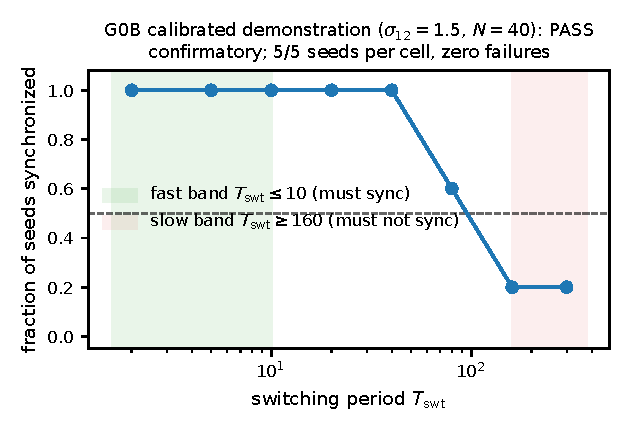
\includegraphics[width=0.6\linewidth]{fig_g0b_sync_fraction.pdf}
  \caption{G0B synchronization fraction versus switching period (confirmatory).
  The frozen criterion constrains only the shaded bands.}
  \label{fig:g0b}
\end{figure}

\paragraph{G0C: INCONCLUSIVE (confirmatory).}
Transverse contraction exists: $\Psi<0$ across the entire frozen grid (at the
fastest $\Tswt=11$: $\Psi=-0.008$ at $\sigma=0.05$ down to $-0.177$ at
$\sigma=0.8$). But the stability onset is $\sigma=0.05$ --- the smallest grid
value --- at \emph{every} $\Tswt\in\{11,25,100,135\}$, so no switching-time
dependence was resolved on the frozen grid
(PARTIAL\_NO\_TSWT\_DEPENDENCE). Descriptively, contraction is present;
confirmatorily, the $\Tswt$-dependence that the translation needs was not
shown at this resolution.

\paragraph{G1-weak: INCONCLUSIVE / TIE (confirmatory).}
The rate arm selected on the frozen selection seeds was \emph{fast}
(selection scores: fast $+0.0366$, intermediate $+0.0071$, slow $-0.0155$).
On the eight disjoint evaluation seeds, all eight paired differences
$\gamma_{\mathrm{arm}}-\gamma_{\mathrm{static}}$ are positive (sign test
$p=0.0078$), but the mean $+0.0420$ lies inside the preregistered band
$b=0.0666$ (Figure~\ref{fig:g1g2}, left). Under the frozen rule this is
INCONCLUSIVE (TIE): \textbf{directional evidence exists, but the effect failed
the preregistered magnitude criterion.} We do not reinterpret this as a pass.

\paragraph{G1-strict and G2: NOT\_INTERPRETABLE (diagnostic only).}
Because G1-weak did not pass, the frozen hierarchy renders G1-strict and G2
non-interpretable; we report their values strictly as diagnostics
(Figure~\ref{fig:g1g2}, middle and right; Table~\ref{tab:inference}).
Diagnostically, the G1-strict differences
$\gamma_{\mathrm{arm}}-\max(\gamma_{\mathrm{avg}},\gamma_{\mathrm{best\,static}})$
are negative in \emph{all eight} evaluation seeds (mean $-0.0046$): the
switching arm never beat the aggregate comparator in this ensemble. The G2
order statistic is small ($+0.0030$) and not significant ($p=0.070$). These
diagnostics must not be promoted to confirmatory conclusions --- in either
direction.

\begin{figure}[t]
  \centering
  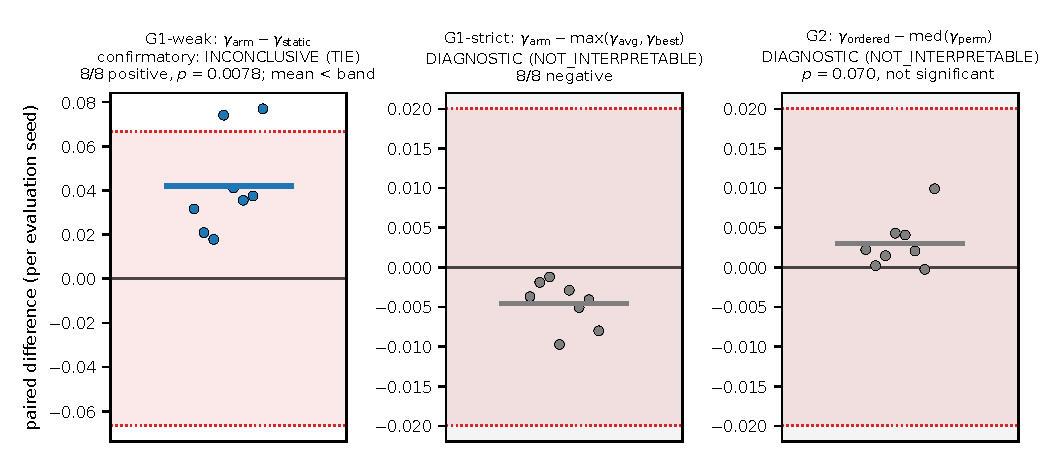
\includegraphics[width=0.98\linewidth]{fig_g1g2_paired_differences.pdf}
  \caption{Per-seed paired differences with preregistered effect bands (red).
  Left: confirmatory G1-weak. Middle/right (grey background): diagnostic
  G1-strict and G2, NOT\_INTERPRETABLE under the frozen hierarchy.}
  \label{fig:g1g2}
\end{figure}

\paragraph{G3: INCONCLUSIVE (confirmatory).}
Every stage shows a positive mean advantage
$\gamma_{\mathrm{fast}}-\gamma_{\mathrm{static}}$ (from $+0.0455$ to
$+0.0631$), with $8/8$ positive signs in four of five stages --- yet no stage
exceeds its frozen band (Figure~\ref{fig:g3}, Table~\ref{tab:inference}), and
the gate requires the faithful and mild-heterogeneity stages to pass. The
signed stage satisfied its implementation prerequisites (per-seed negative
weights present; Frobenius budget matched to $10^{-9}$), so the verdict is a
clean INCONCLUSIVE, not an execution artifact.

\begin{figure}[t]
  \centering
  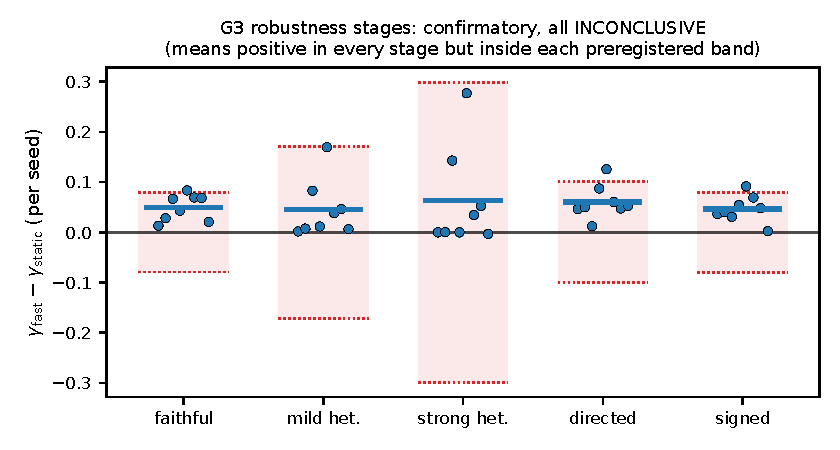
\includegraphics[width=0.78\linewidth]{fig_g3_stages.pdf}
  \caption{G3 per-stage paired differences with per-stage effect bands
  (confirmatory; all stages INCONCLUSIVE).}
  \label{fig:g3}
\end{figure}

\paragraph{G4: FAIL (confirmatory).}
The factor-free basis estimator recovers the active channel set with
precision $=$ recall $=0.353$ under synchronous observation and $0.254$ under
asynchronous/LOCF observation --- far below the preregistered $0.6$ bar
(Figure~\ref{fig:g4}). It does beat the factor-confounded baseline
(margin $+0.162$, band $0.065$, $8/8$ positive, $p=0.0078$) and, under
synchronous sampling, tracks contraction well (correlation $0.948$). Under
asynchronous/LOCF sampling the contraction correlation collapses to $0.010$
--- an Epps-like degradation \citep{epps1979comovements,scholes1977estimating},
consistent with the classical observation that asynchronous sampling destroys
short-horizon comovement estimates even when consistent estimators exist
\citep{hayashi2005covariance}. Two of the four frozen conditions fail, so the
gate fails.

\begin{figure}[t]
  \centering
  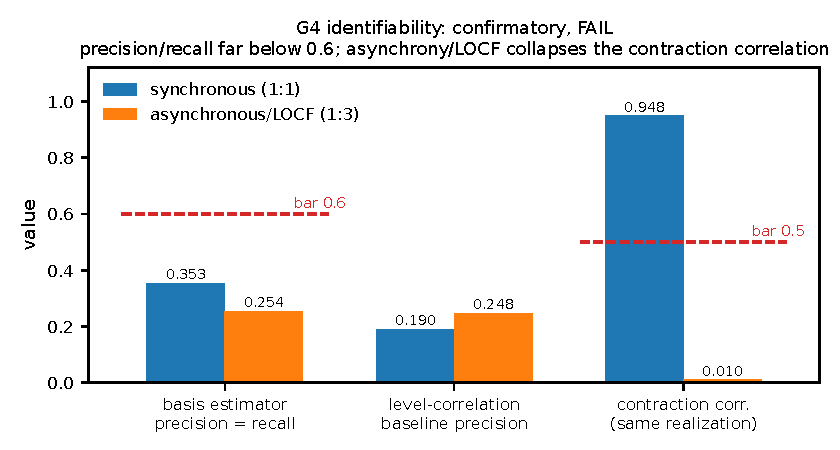
\includegraphics[width=0.72\linewidth]{fig_g4_identifiability.pdf}
  \caption{G4 identifiability metrics under synchronous (1:1) and
  asynchronous/LOCF (1:3) observation (confirmatory; gate FAIL).}
  \label{fig:g4}
\end{figure}

% Decision statistics, transcribed from the frozen JSON reports (attempt
% 1baa47da06fede2a). band = max(3 * sample sd (ddof=1), preregistered floor).
\begin{table}[t]
\centering
\caption{Paired decision statistics ($n=8$ evaluation seeds per test; exact
two-sided sign test on non-zero differences; effect band
$b=\max(3\,\hat{\sigma}_{\mathrm{ddof}=1},\,\text{floor})$; floors: $0.02$ for
surrogate $\gamma$, $0.05$ for the identifiability margin). Rows marked
$\dagger$ are diagnostic (NOT\_INTERPRETABLE under the frozen hierarchy).}
\label{tab:inference}
\resizebox{\linewidth}{!}{%
\begin{tabular}{@{}lrrrrl@{}}
\toprule
Test & mean $\bar d$ & band $b$ & signs $(+/-)$ & $p$ & verdict \\
\midrule
G1-weak: $\gamma_{\mathrm{arm}}-\gamma_{\mathrm{static}}$ & $+0.0420$ & $0.0666$ & $8/0$ & $0.0078$ & INCONCLUSIVE (TIE) \\
G1-strict$^\dagger$: $\gamma_{\mathrm{arm}}-\max(\gamma_{\mathrm{avg}},\gamma_{\mathrm{best}})$ & $-0.0046$ & $0.0200$ & $0/8$ & $0.0078$ & (diagnostic) \\
G2$^\dagger$: $\gamma_{\mathrm{ord}}-\mathrm{med}(\gamma_{\mathrm{perm}})$ & $+0.0030$ & $0.0200$ & $7/1$ & $0.0703$ & (diagnostic) \\
\midrule
G3 faithful & $+0.0492$ & $0.0789$ & $8/0$ & $0.0078$ & INCONCLUSIVE (TIE) \\
G3 mild heterogeneity & $+0.0455$ & $0.1715$ & $8/0$ & $0.0078$ & INCONCLUSIVE (TIE) \\
G3 strong heterogeneity & $+0.0631$ & $0.2984$ & $6/2$ & $0.2891$ & INCONCLUSIVE (NOT\_SIG.) \\
G3 directed & $+0.0603$ & $0.1006$ & $8/0$ & $0.0078$ & INCONCLUSIVE (TIE) \\
G3 signed & $+0.0467$ & $0.0799$ & $8/0$ & $0.0078$ & INCONCLUSIVE (TIE) \\
\midrule
G4 beats-baseline margin & $+0.1625$ & $0.0646$ & $8/0$ & $0.0078$ & PASS (condition; gate FAILs on P/R) \\
\bottomrule
\end{tabular}}
\end{table}


\paragraph{G0A: NOT\_RUN (permanent decision).}
The exact paper-scale reproduction ($\sigma_{12}=0.1$, $N$ up to $400$,
$4{,}000$ time units per cell) is outside the authorized cheap-suite scope and
is recorded permanently as NOT\_RUN --- \emph{outside the cheap-suite scope and
unnecessary for the financial-translation decision}. It could be conducted
only as a separate replication project; whatever its outcome, it cannot rescue
G1--G4 (which concern translation, order effects and identifiability, not the
mechanism's existence) and cannot authorize real-market research under the
closed preregistration.

\section{Why the Results Favor an Aggregate-Connectivity Interpretation}
\label{sec:aggregate}

The pattern of outcomes is exactly what fast-switching averaging theory
predicts for this ensemble. The selected arm was the \emph{fastest}; blinking
and fast-switching results
\citep{belykh2004blinking,stilwell2006sufficient,hasler2013dynamics} say that
in this regime the switched system inherits the stability of the
time-averaged network, with finite-rate corrections. Consistently: the weak
advantage over an equal-density \emph{static sparse} graph is directionally
positive (a static sparse subset is simply a worse average), while the
diagnostic strict comparison against the average-graph operator is negative in
every seed. Nothing in the confirmatory record shows switching delivering
anything \emph{beyond} its time-average here.

Two disciplined qualifications. First, this is not an impossibility claim:
designed temporal networks can provably outperform static ones under resource
constraints \citep{zhang2021designing}, and our frozen ensemble was not
designed to sit in that regime; the negative reading applies to this
preregistered ensemble, not to all switching systems. Second, the G2
permutation-median comparator aggregates signed order effects across seeds and
can cancel sign-varying order effects; this limitation was frozen and
disclosed in advance.

For finance the implication is direct: under this translation, measured
``switching structure'' carried no confirmed information beyond the average
network. Aggregate connectedness measures
\citep{diebold2009measuring,diebold2014network,billio2012econometric} --- and
time-varying correlation models \citep{engle2002dynamic} with the usual
heteroskedasticity discipline \citep{forbes2002no} --- already target that
average object. A switching-based market study would therefore need to
demonstrate, first and preregistered, an effect beyond the average graph;
ours did not.

\section{Observational Identifiability and Asynchrony}
\label{sec:identifiability}

Under synthetic conditions more favorable than those normally available in
empirical finance --- known dynamics, same-realization ground truth, a
factor-free estimator by construction, and synchronous noise-controlled
observations --- channel-set recovery reached precision and recall of only
$0.353$. Beating the
factor-confounded baseline (margin $+0.162$; the baseline's precision is
$0.190$) confirms that venue differencing removes the common factor, in the
spirit of factor-removal approaches
\citep{fan2013large,barigozzi2017network}, but ``better than a confounded
baseline'' is far from ``reliable''. Under asynchronous/LOCF observation at a
modest 1:3 ratio, recovery degrades further ($0.254$) and the contraction
correlation collapses from $0.948$ to $0.010$. We stress the frozen
terminology: this is an \emph{asynchrony/LOCF (Epps-like degradation)}
experiment --- it reproduces the practical consequence highlighted by
\citet{epps1979comovements} in our setting; it is not a causal demonstration
of the Epps effect, and estimators designed for non-synchronous data
\citep{hayashi2005covariance,scholes1977estimating} were not the object under
test. Since real markets add unknown dynamics, latent factors, microstructure
noise and far harsher asynchrony, the preregistered conclusion is that the
mechanism's observational signature is not reliably identifiable in this
class of designs; a real-data ``detection'' built on such an estimator would
not be interpretable.

\section{Limitations}
\label{sec:limitations}

\begin{enumerate}
  \item \textbf{Scope of the negative result.} All conclusions are relative to
  the frozen ensemble, grids and decision contract. We did not search
  parameter space for regimes where switching beats the average
  \citep{zhang2021designing}; that would be a different, new preregistration.
  \item \textbf{Small $n$, wide bands.} With $n=8$ paired seeds and a
  $3\hat{\sigma}$ band, magnitude criteria are conservative; consistent
  directional effects (8/8 signs) can land INCONCLUSIVE, as G1-weak and four
  G3 stages did. This is by design (anti-inflation), but it limits power.
  \item \textbf{Comparator strength.} G1-strict uses the best of a frozen
  248-candidate static set, not the best admissible static subset
  ($\binom{24}{6}=134{,}596$); claims about the true static optimum are
  impossible and none are made.
  \item \textbf{G2 statistic.} The permutation-median comparator detects a
  systematic displacement from the permutation median; sign-varying order
  effects across seeds can cancel (frozen, disclosed limitation).
  \item \textbf{G0C resolution.} The onset grid starts at $\sigma=0.05$ and
  the onset saturated at that smallest value for every $\Tswt$; a finer grid
  might resolve dependence. The minimal $N=2$ construction is also the
  weakest link to the full spatiotemporal system.
  \item \textbf{G0A not run.} The exact paper-scale reproduction was not
  executed; G0B is a calibrated demonstration at different coupling and size
  and cannot substitute for it.
  \item \textbf{The surrogate is not a market model.} It is a mechanism
  testbed. No claim about real markets, trading, price prediction or market
  causality follows from any result here --- positive or negative. No real
  market data were used anywhere.
\end{enumerate}

\section{Reproducibility and Audit Trail}
\label{sec:repro}

The study enforced preregistration-grade custody end to end:
(i) scientific preregistration and operational execution contract, versioned
and bound by canonical hashes (v8/v6 at execution);
(ii) a content-addressed freeze manifest over all code, configuration, tests
and documents (117 files), whose stored content hash equals independent
recomputation;
(iii) a single authorized execution from the freeze commit with a clean tree,
identified by an authorization token recorded only as its SHA-256, producing
attempt \texttt{1baa47da06fede2a};
(iv) a sealed attempt directory whose manifest inventories every artifact by
size and SHA-256 and whose seal equals the manifest content hash;
(v) a separate post-execution artifact audit that reconstructed the package
and recomputed all identities, hashes and decision statistics exactly;
(vi) byte-for-byte custody of the sealed outputs in the repository under an
annotated tag, distinct from the execution freeze commit.
Every figure and table in this paper is generated from the frozen JSON
reports without re-running any simulation. Earlier execution freezes v2--v7
were each found non-executable by separate pre-execution artifact audits and
were \emph{never run}; consequently no result predates the sealed attempt. All identifiers
appear in Appendix~\ref{app:audit}.

\section{Conclusion}
\label{sec:conclusion}

SwitchSync Markets demonstrates the switching-synchronization mechanism in a
calibrated synthetic setting (G0B PASS), but under the preregistered criteria
it does not establish an advantage beyond aggregate connectivity (G1-weak
INCONCLUSIVE/TIE; G1-strict diagnostic and non-interpretable), a robust
temporal-order effect (G2 non-interpretable; G3 INCONCLUSIVE), or reliable
observational identifiability (G4 FAIL). The financial translation is
therefore not supported for empirical or operational development under the
preregistered criteria: no predictive or operational market study is
justified, and no trading signal, backtest, PnL, Sharpe or deployment claim
exists or is implied. No real market data were used. This outcome does not
refute the mathematical results of the seed paper
\citep{eser2025switching}; it delimits what that mechanism can currently be
expected to deliver as a measurable, decision-relevant object in financial
data, and it documents --- with full custody --- how a preregistered negative
result of this kind can be produced and audited.

\section*{Transparency Statement}

Generative-AI systems assisted with code generation, testing, artifact
auditing, and manuscript drafting. The human author reviewed the scientific
claims and assumes full responsibility for the submitted work.

\appendix

\section{Audit and Reproducibility Appendix}
\label{app:audit}

\paragraph{Identifiers.} Table~\ref{tab:audit} lists the immutable hashes.
The execution scope was \texttt{cheap-suite}; G0A is permanently NOT\_RUN.
The authorization token is recorded only as its SHA-256:
\begin{center}
\footnotesize\texttt{3b4b903518fa5cb337cbf5416aa8cc6db8db47c1548b39545f562158b07aca29}
\end{center}
\noindent the attempt id satisfies
$\mathrm{attempt}=\mathrm{sha256}(\mathrm{campaign}\,\|\,\mathrm{scope}\,\|\,\mathrm{token\_sha})[:16]$,
so an auditor recomputes it without the raw token. Zero failure records,
non-finite values or dropped seeds occurred. No real data were accessed.

% Audit / reproducibility identifiers (Appendix A). All values verified by an
% independent audit of the sealed attempt.
\begin{table}[h]
\centering
\caption{Immutable identifiers of the preregistration, the execution freeze and the
sealed result. Earlier execution freezes v2--v7 were each found non-executable by
independent audit and were \emph{never run}; no result predates the attempt below.}
\label{tab:audit}
\resizebox{\linewidth}{!}{%
\begin{tabular}{@{}ll@{}}
\toprule
Object & SHA-256 / identifier \\
\midrule
prereg v8 (canonical) & \texttt{a667434d0d7c5905d62cf81b79699f2799e2597128631cab1e4792bed6053dd9} \\
prereg v8 (file) & \texttt{896163891b8b43f42511a1a57294d6075f3b65f33877780daf82cc03a54d568e} \\
execution contract v6 (canonical) & \texttt{6dbe79ddf1d0b6e5e63f74a5ae3ed947abfc837419f4b7938fdcf8c09f525ee8} \\
execution contract v6 (file) & \texttt{80609ef5a90817813f0a9978ec017ab00734c3681abb0429fbe4ec4582b8c2bb} \\
execution freeze v8 (content hash) & \texttt{2991e064ced6154c149fa57d4fc77e855bede51750565c264972b369778d112d} \\
freeze commit (= runtime HEAD) & \texttt{5ca40c7da87f583c7cea1cefd00cc978c3731d98} \\
result-custody commit & \texttt{48339e47d3a0911949cf25c83a50e63fc9572aa5} \\
campaign / attempt id & \texttt{44be3a5d07e67b5e} / \texttt{1baa47da06fede2a} \\
manifest content hash (= SEALED) & \texttt{4e029d814437695d99c4b5cc62cbe3cf94ebd0e46c6e9ae51d54cc5f28f3c33d} \\
\midrule
\texttt{g0b\_calibrated\_v2.json} & \texttt{d592b75d59b6e50c51ec6263c0a8469654651e0ef247fd2fadd3cf5adad4d4e5} \\
\texttt{g0c\_msf\_v2.json} & \texttt{150a53dc42236742d347012704a00a4d2e1db52d99bb800341bbc3ec6de484d0} \\
\texttt{g1\_g2\_paired\_v2.json} & \texttt{b6242cd72510ce6d8b0daa5edba31b1c124f3fa519eae92ac0a408f06decbce0} \\
\texttt{g3\_robustness\_v2.json} & \texttt{2f16a4578c5b48cbb8621455b5a37042ec615a7127c9d709acb43ab1a3414964} \\
\texttt{g4\_identifiability\_v2.json} & \texttt{bd148d1ed23ba057df41dedfbdb7414b7d450a7f5c28b59617e354d5bbb597e6} \\
\bottomrule
\end{tabular}}
\end{table}


\paragraph{Seed blocks (frozen in prereg v8).}
chaos $\{7\}$; G0A $\{11,12,13\}$; G0B $\{11,\dots,15\}$; G0C $\{31\}$;
paired selection $\{41,\dots,48\}$; paired evaluation $\{81,\dots,88\}$;
G3 stages $\{51,\dots,58\}$; identifiability $\{61,\dots,68\}$.

\paragraph{Environment (pinned and verified at execution).}
Python 3.14.3; numpy 2.4.4; scipy 1.17.1; matplotlib 3.10.9; Linux x86-64
(glibc 2.35); RK4 with $\mathrm{d}t=0.01$; runtime $\approx 8$\,min\,44\,s for
the full cheap suite.

\paragraph{Execution history declaration.}
Execution freezes v2--v7 were each found non-executable by separate
pre-execution artifact audits (defects ranged from custody flaws to a missing
frozen tolerance block) and were superseded without ever producing a result. The
sealed attempt \texttt{1baa47da06fede2a} under freeze v8 is the \emph{only}
scientific execution of this project.

\section{Frozen Decision Details}
\label{app:decisions}

\paragraph{Shared rule.} Exact two-sided sign test on non-zero paired
differences at $\alpha=0.05$; effect band
$b=\max(3\hat{\sigma}_{\mathrm{ddof}=1},\text{floor})$; PASS/FAIL only outside
$\pm b$; bootstrap (2{,}000 resamples, frozen seed 20260713) reported as
descriptor only.

\paragraph{G1/G2 selection protocol.} Arm and best-static comparator selected
on the selection seed block only, using a common per-seed validity mask over
\emph{all} rate arms and \emph{all} 248 static candidates, then frozen before
evaluation seeds are opened. Ties break canonically (arm order
fast$<$intermediate$<$slow; lexicographic subsets).

\paragraph{G4 conditions (all four required).} mean precision $>0.6$;
mean recall $>0.6$; same-realization contraction correlation $>0.5$;
significant positive margin over the factor-confounded baseline (floor
$0.05$). Observed: $0.353$; $0.353$; $0.948$ (synchronous); margin $+0.162$
(PASS) --- two conditions fail, hence gate FAIL.

\bibliographystyle{plainnat}
\bibliography{references}

\end{document}
